\documentclass{article}
\usepackage[utf8]{inputenc}
\usepackage[english]{babel}
\usepackage{hyperref}
\usepackage{graphicx}

\title{Interim Report WV}
\author{Ward  Xavier}
\date{March 2015}


\begin{document}
\maketitle

\section{Update}
Due neverending problems with over-the-air-deployment we decided to stop researching using Looci. We are now using just Contiki on the motes. We deploy components with the flasher.
\section{Interim Results}
In general all the results that we get from the OC and process with the Matlab script are negative. To interpret the results we just filipped the sign.
\subsection{RAM}
We wrote a component that writes 100 times 8kB to the RAM-memory, it repeats this action infinite times. Between the repetition the mote does nothing and is idle. We used the OC to measure a certain interval en we got the following results:\\
\\
-71.4368 -232.0165  -71.4722 -231.9092  -71.4422 -231.8196  -71.5196 -231.8710  -71.5787 -231.8401  -71.5961 -232.0866  -71.4173 -232.1306  -71.5185 -231.8660  -71.4893 -231.7818  -71.4970
\\
Energy when idle: $\pm 71 mj$\\
Energy when writing: $\pm 231 mj$
\subsection{Antenna}
\subsubsection{Enegry/byte}
We used the data provided at \url{http://people.cs.kuleuven.be/~wilfried.daniels/energy/results3.html} and used it to derive the energy cost per byte:
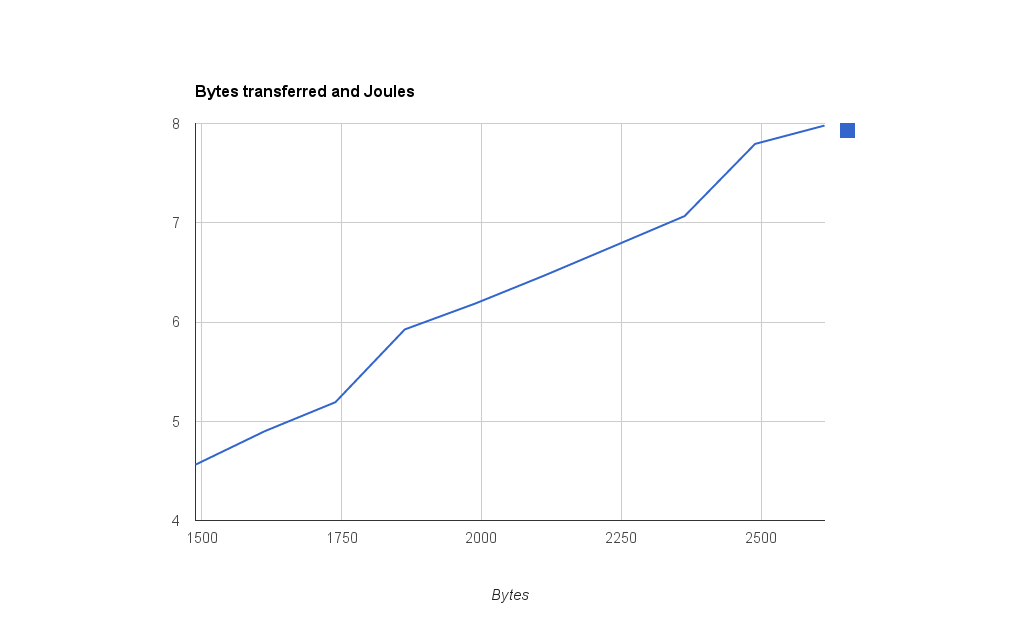
\includegraphics[width=\linewidth]{graph.png}
The average cost was: $0.00306399592 J/Byte.$
\subsubsection{Other aspects}
Next we also wanted to know the usage when the mote is listening and when it is idle. We wrote  a component that did nothing (with the antenna explicit off) and just used the pinflips, and anther with the antenna explicit on.
\subsubsection{Enegry when idle}
We got about the same energy usage as during the ram test when we wrote nothing:\\
-74.7316  -74.7610  -74.7003  -74.6391  -74.4582  -74.6195  -74.6579  -74.4509  -74.6454  -74.7656  -74.5681  -74.8548  -74.6121  -74.7943  -74.8279  -74.8777  -74.6717  -74.9203\\
\\
However as you can notice there is a tiny difference and we are not certain what the cause is?
\subsubsection{Enegry when listening}
During the listening test we got the following results:\\
-114.8897 -114.8994 -114.8356 -115.1350 -115.1103 -114.9205 -115.2339 -115.2512 -115.1336 -115.2102 -115.0942 -115.0485 -115.2242 -115.2833 -115.1356 -115.3479 -115.2736 -115.0013\\
\subsection{Energy to start the antenna}
%TODO 
\subsection{Flash}
As discussed with Klaas, we will only research this option when we have time.

\subsection{Interim Conclusion}
%TODO

\section{Questions}
\begin{itemize}
\item The results from our measurements, are they correct?
\item 
\end{itemize}
\end{document}
